\documentclass[twocolumn, 10pt]{article}

\usepackage{amsmath}
\usepackage{graphicx}
\usepackage{float}
\graphicspath{ {./images/} }

\title{2XC3 - Lab 1 Report}
\author{Oleg Glotov\\ L03, 400174037\\ glotovo@mcmaster.ca \and Emma Willson\\ L02, 400309856\\ willsone@mcmaster.ca}


\begin{document}
\maketitle
\section{Git Setup}\label{sec:git}
The group began by setting up out github accounts and the repository. The visibility was set to private to comply with McMaster's code of conduct.

\begin{figure}[H]
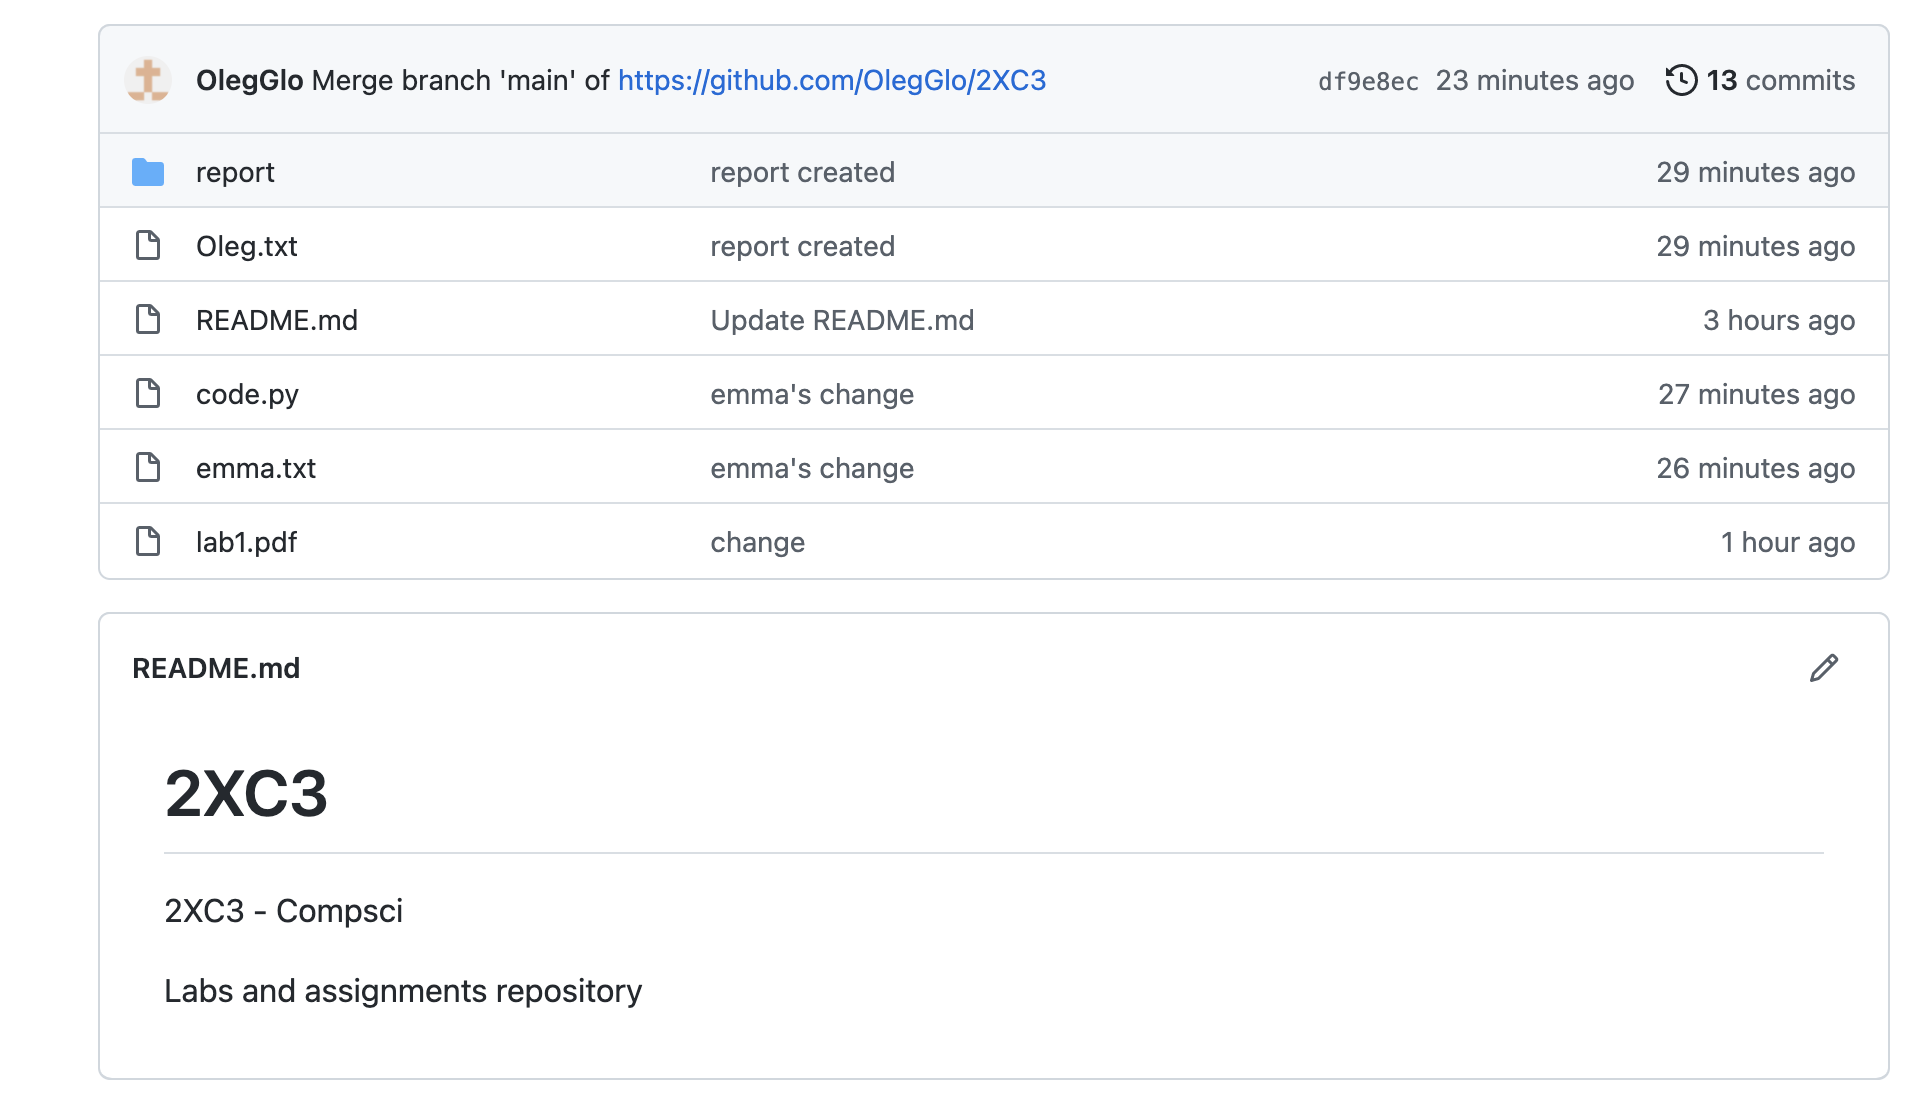
\includegraphics[width=\linewidth]{img1}
\end{figure}

Both of us has access to the repository. We choose to work with github directly thorough our VSCode IDE since it fully integrates git commands and simplifies the workflow.

\section{Git commands}

Here we fucked around more resulting in the shit you see below

Write up revert and reset

and

The

other 

things

Merge demo

\begin{figure}[H]
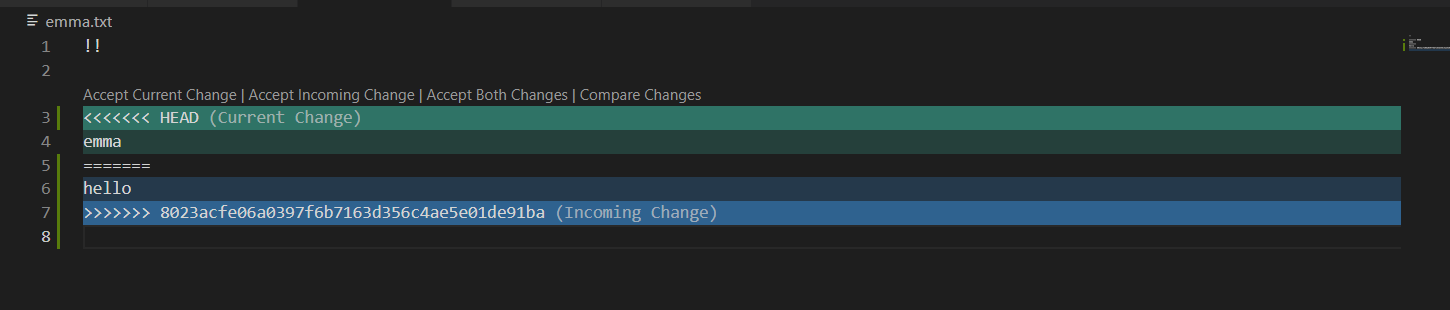
\includegraphics[width=\linewidth]{merge}
\end{figure}

\section{Code.py}

Both group member's code is provided below. After consulting we decided to combine both of ours solution into the final product in the file code.py not provided here.

Oleg's version:

\footnotesize
\begin{verbatim}
def are_valid_groups(groups, studentNum):

    length = len(studentNum)
    count = 0
    
    for group in groups:
        count = 0
        for students in studentNum:
            if (group.count(students) == 0):
                break
            if (group.count(students) == 1):
                count += 1
        
        if count == length:
            return True
        
    return False

print(are_valid_groups(groups, studentNum))
\end{verbatim}
\normalsize

Emma's version:

\footnotesize
\begin{verbatim}
def are_valid_groups(groups, studentNum):

    length = len(studentNum)
    count = 0
    
    for group in groups:
        count = 0
        for students in studentNum:
            if (group.count(students) == 0):
                break
            if (group.count(students) == 1):
                count += 1
        
        if count == length:
            return True
        
    return False

print(are_valid_groups(groups, studentNum))
\end{verbatim}
\normalsize

\section{Player vs Adversary}
Let the games begin
\end{document}

